\section{System Tests}
\subsection{Ping Test}

\begin{figure}[H]
  \centering
  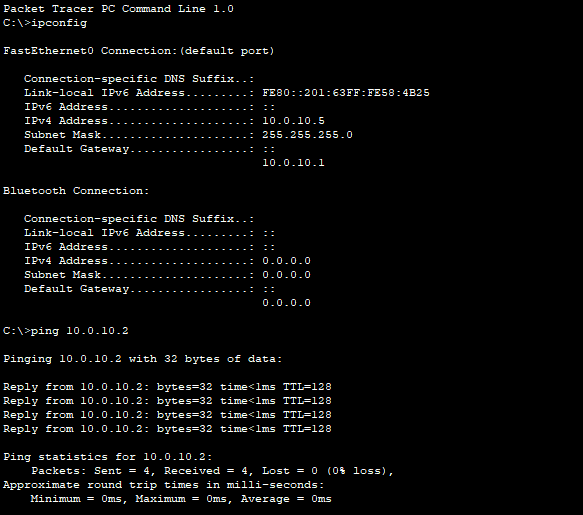
\includegraphics[width=0.4\textwidth]{./assets/ping.hqw-hqw.png}
  \caption{Ping between workstations at HQ}
\end{figure}

\begin{figure}[H]
  \centering
  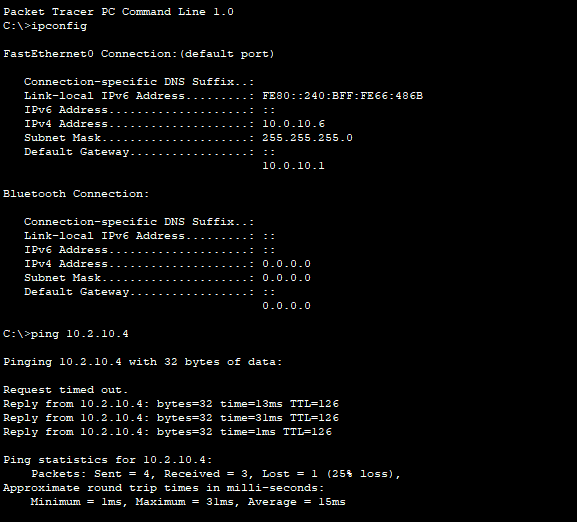
\includegraphics[width=0.4\textwidth]{./assets/ping.hqw-dnw.png}
  \caption{Ping from HQ workstation to DN workstation}
\end{figure}

\begin{figure}[H]
  \centering
  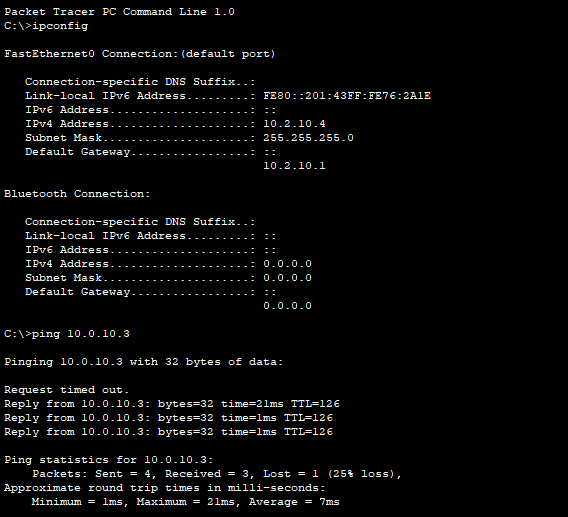
\includegraphics[width=0.4\textwidth]{./assets/ping.dnw-hqw.png}
  \caption{Ping from DN workstation to HQ workstation}
\end{figure}

\begin{figure}[H]
  \centering
  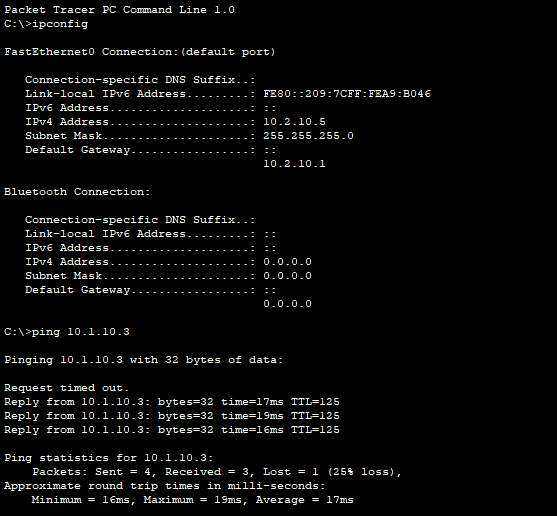
\includegraphics[width=0.4\textwidth]{./assets/ping.dnw-ntw.png}
  \caption{Ping from DN workstation to NT workstation}
\end{figure}

\begin{figure}[H]
  \centering
  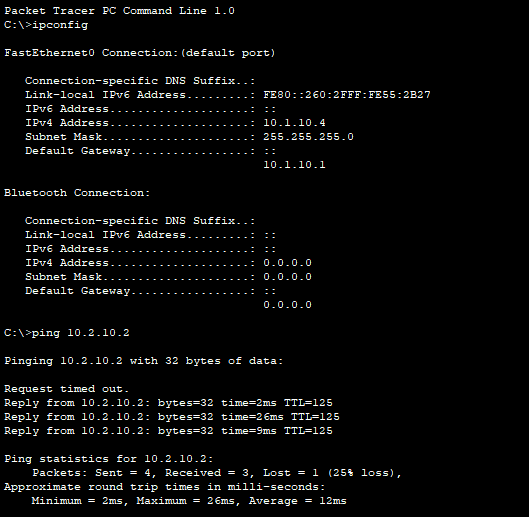
\includegraphics[width=0.4\textwidth]{./assets/ping.ntw-dnw.png}
  \caption{Ping from NT workstation to DN workstation}
\end{figure}

\begin{figure}[H]
  \centering
  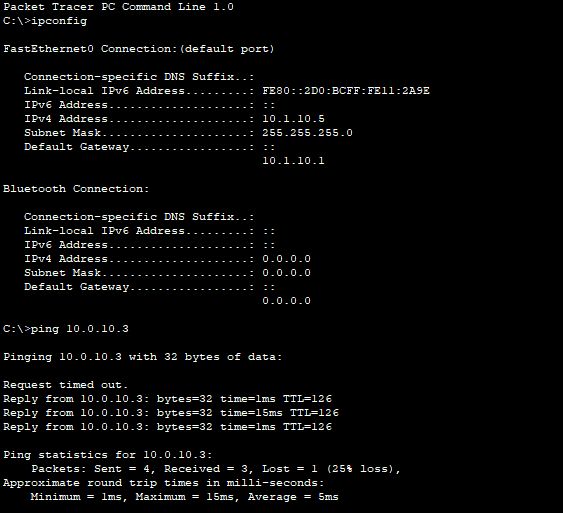
\includegraphics[width=0.4\textwidth]{./assets/ping.ntw-hqw.png}
  \caption{Ping from NT workstation to HQ workstation}
\end{figure}

\begin{figure}[H]
  \centering
  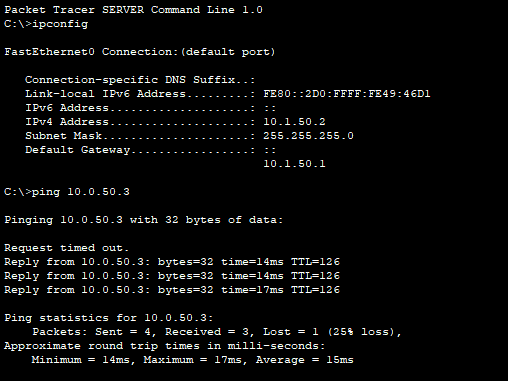
\includegraphics[width=0.4\textwidth]{./assets/ping.nts-hqs.png}
  \caption{Ping from NT server to HQ server}
\end{figure}

\begin{figure}[H]
  \centering
  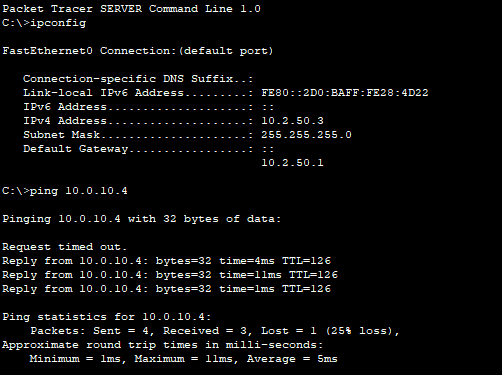
\includegraphics[width=0.4\textwidth]{./assets/ping.dns-hqw.png}
  \caption{Ping from DN server to HQ workstation}
\end{figure}

\begin{figure}[H]
  \centering
  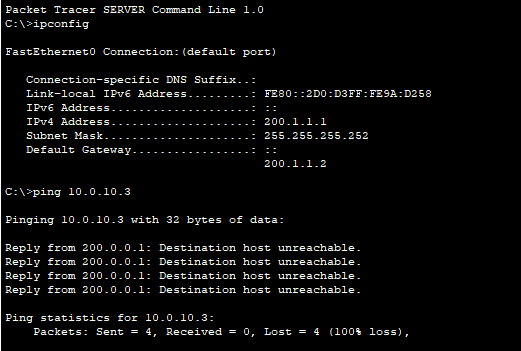
\includegraphics[width=0.4\textwidth]{./assets/ping.web-hqw.png}
  \caption{Ping from internet to HQ workstation}
\end{figure}

\begin{figure}[H]
  \centering
  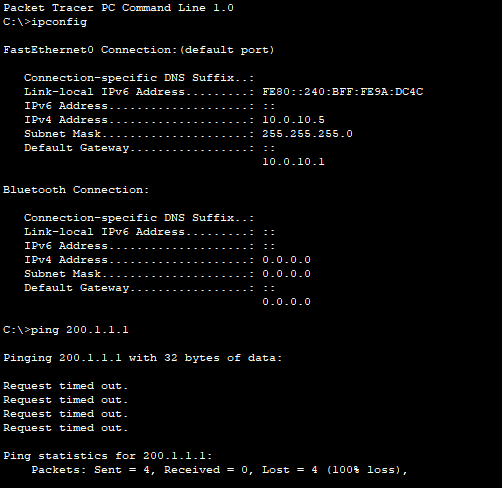
\includegraphics[width=0.4\textwidth]{./assets/ping.hqw-web.png}
  \caption{Ping from HQ workstation to internet}
\end{figure}

\begin{figure}[H]
  \centering
  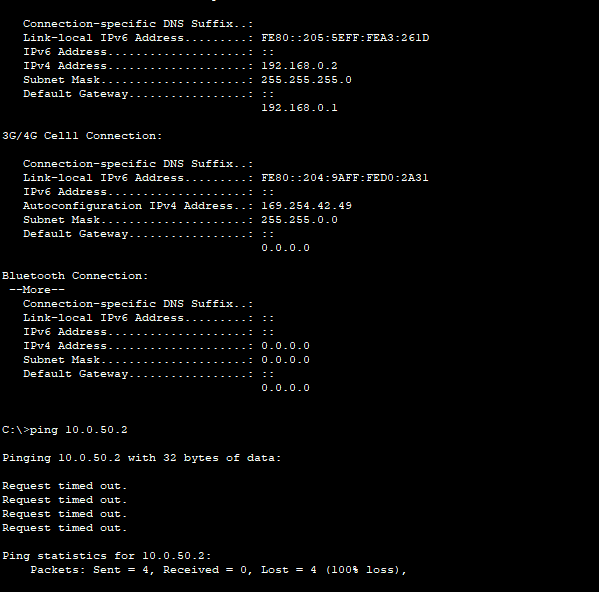
\includegraphics[width=0.4\textwidth]{./assets/ping.hqp-hqs.png}
  \caption{Ping from HQ phone to HQ server}
\end{figure}

\begin{figure}[H]
  \centering
  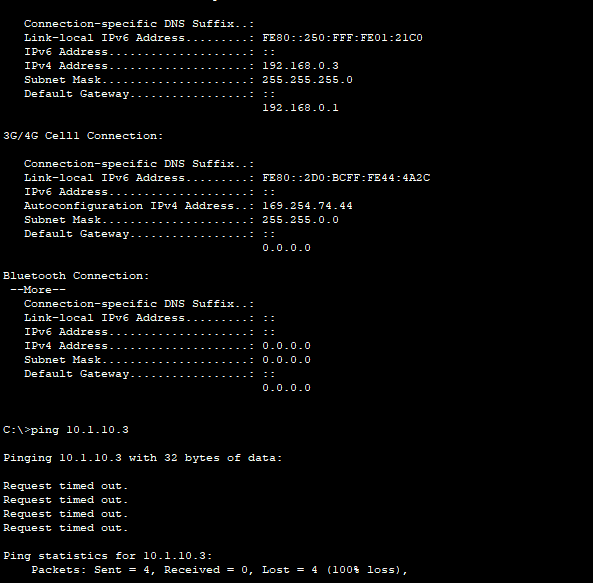
\includegraphics[width=0.4\textwidth]{./assets/ping.hqp-ntw.png}
  \caption{Ping from HQ phone to NT workstation}
\end{figure}

\begin{figure}[H]
  \centering
  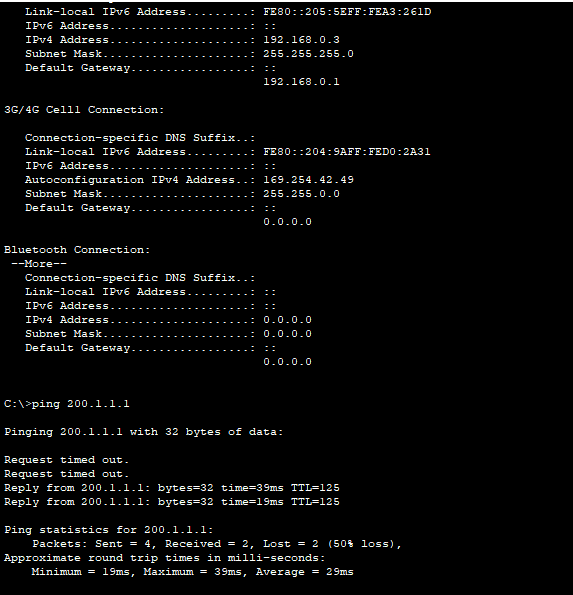
\includegraphics[width=0.4\textwidth]{./assets/ping.hqp-web.png}
  \caption{Ping from HQ phone to internet}
\end{figure}

\begin{figure}[H]
  \centering
  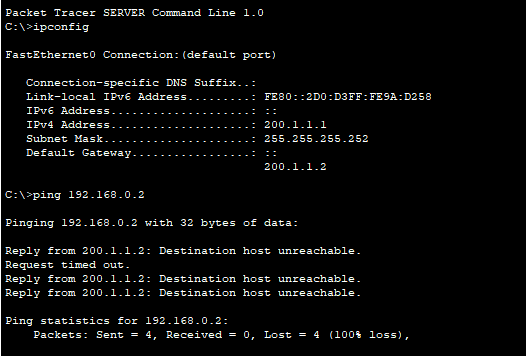
\includegraphics[width=0.4\textwidth]{./assets/ping.web-p.png}
  \caption{Ping from internet to NT phone}
\end{figure}

\begin{figure}[H]
  \centering
  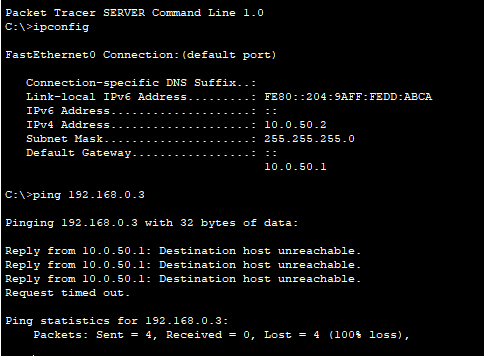
\includegraphics[width=0.4\textwidth]{./assets/ping.hqs-hqp.png}
  \caption{Ping from HQ server to HQ phone}
\end{figure}

You might have noticed that the first try of some ping commands fails.
That is due to the switches not having a route cached.

\subsection{Traceroute Test}
\begin{figure}[H]
  \centering
  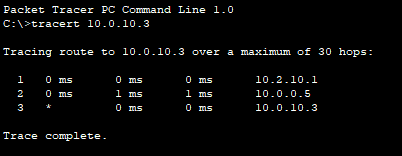
\includegraphics[width=0.4\textwidth]{./assets/trace.dnw-hqw.png}
  \caption{Tracert from DN workstation to HQ workstation}
\end{figure}

\begin{figure}[H]
  \centering
  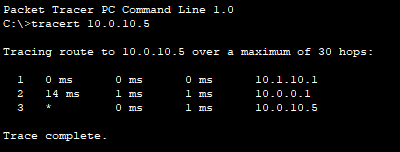
\includegraphics[width=0.4\textwidth]{./assets/trace.ntw-hqw.png}
  \caption{Tracert from NT workstation to HQ workstation}
\end{figure}

\begin{figure}[H]
  \centering
  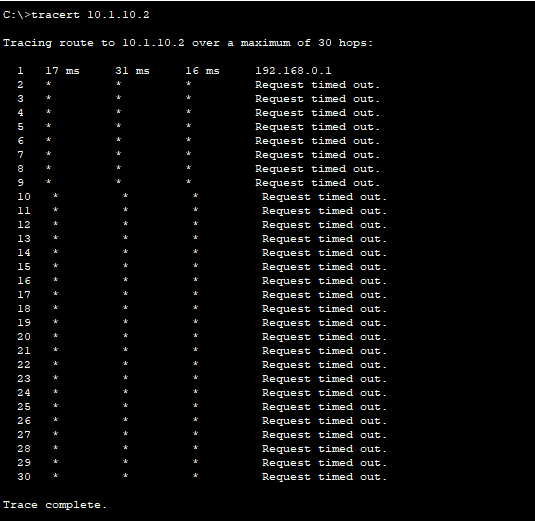
\includegraphics[width=0.4\textwidth]{./assets/trace.hqp-ntw.png}
  \caption{Tracert from HQ phone to NT workstation}
\end{figure}

\subsection{MAC Address Table and OSPF IP Table}
\begin{figure}[H]
  \centering
  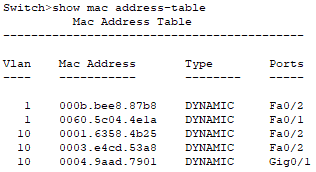
\includegraphics[width=0.4\textwidth]{./assets/mac.hqw.png}
  \caption{MAC address table of workstation switch at HQ}
\end{figure}

\begin{figure}[H]
  \centering
  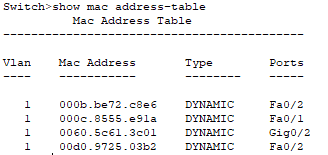
\includegraphics[width=0.4\textwidth]{./assets/mac.ntw.png}
  \caption{MAC address table of workstation switch at NT branch}
\end{figure}

\begin{figure}[H]
  \centering
  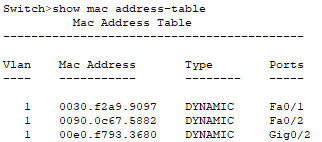
\includegraphics[width=0.4\textwidth]{./assets/mac.dnw.png}
  \caption{MAC address table of workstation switch at DN branch}
\end{figure}

\begin{figure}[H]
  \centering
  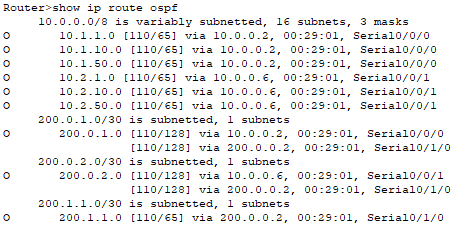
\includegraphics[width=0.4\textwidth]{./assets/ospf.hq.png}
  \caption{OSPF IP table at HQ}
\end{figure}

\begin{figure}[H]
  \centering
  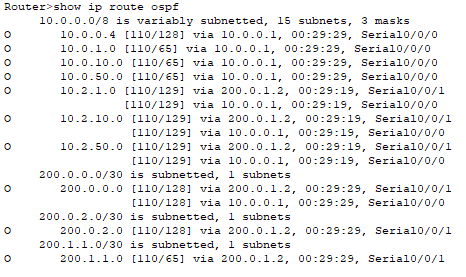
\includegraphics[width=0.4\textwidth]{./assets/ospf.nt.png}
  \caption{OSPF IP table at NT branch}
\end{figure}

\begin{figure}[H]
  \centering
  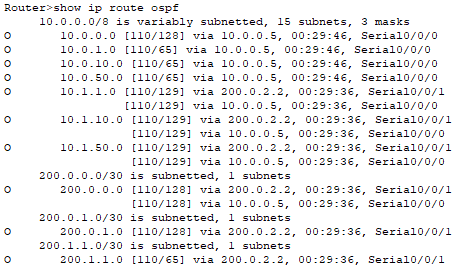
\includegraphics[width=0.4\textwidth]{./assets/ospf.dn.png}
  \caption{OSPF IP table at DN branch}
\end{figure}

The MAC address tables and OSPF IP tables are not anywhere near complete because they are the entries currently cached in the devices.
These tables will expand as more transactions go through these devices.
